% !TEX program = xelatex
\documentclass[10pt, aspectratio=169]{beamer}

\usetheme{metropolis}
\usefonttheme[onlymath]{serif}
\metroset{numbering=fraction}

\usepackage{fontspec}
\setsansfont{Hiragino Sans W3}[BoldFont={Hiragino Sans W6}]

\usepackage{amsmath, amssymb, amsfonts, mathtools}
\usepackage{bm}
\let\oldtextbf\textbf
\renewcommand{\textbf}[1]{\oldtextbf{\boldmath #1}}
\usepackage{tikz}
\usetikzlibrary{cd, arrows.meta, positioning, calc, shapes.geometric, shapes.symbols, fit}
\tikzset{every node/.style={font=\sffamily}}
\usepackage{xcolor}

\definecolor{hilight}{HTML}{DBEAFE}
\definecolor{indigo}{HTML}{4338CA}
\definecolor{epsgreen}{HTML}{16A34A}
\definecolor{iotared}{HTML}{DC2626}

\newcommand{\hl}[1]{\colorbox{hilight}{\(\displaystyle #1\)}}

\definecolor{chipblue}{HTML}{DBEAFE}
\definecolor{chipred}{HTML}{FEE2E2}
\newcommand{\chip}[2][chipblue]{\tikz[baseline=(X.base)]\node[fill=#1, rounded corners=3pt, inner sep=3pt, outer sep=1pt] (X) {\strut #2};}

\title{最近 QFT (場の量子論) に少し入門したので話してみたい}
\author{@dokadokaas}
\date{}

\begin{document}

\maketitle

\begin{frame}{自己紹介}
  \begin{tikzpicture}[remember picture, overlay]
    \node[anchor=north east, inner sep=0pt] at ([xshift=-1cm, yshift=-1.5cm]current page.north east) {
      
\includegraphics[width=3.8cm]{assets/docker-whale.png}
    };
  \end{tikzpicture}
  \begin{itemize}\setlength\itemsep{0.5em}
    \item \textbf{興味ある} \chip{数理物理} \chip{表現論} \chip{作用素環} \chip{確率論}
    \item \textbf{最近} \chip{場の量子論}（今日はその話）
    \item \textbf{興味あるけどわかんなすぎる} \chip[chipred]{整数論} \chip[chipred]{代数幾何}
  \end{itemize}
\end{frame}

\begin{frame}{この発表の流れ}
\begin{center}
\begin{tikzpicture}[
  node distance=0.5cm,
  chapnode/.style={fill=chipblue, rounded corners, inner sep=8pt, font=\large},
  reasonnode/.style={font=\small, text=gray}
]
  \node[chapnode] (kg) {クライン-ゴルドン場};
  \node[reasonnode, below=of kg] (a1) {$\downarrow$ \ 境界項};
  \node[chapnode, below=of a1] (sol) {解空間とシンプレクティック形式};
  \node[reasonnode, below=of sol] (a2) {$\downarrow$ \ 量子化};
  \node[chapnode, below=of a2] (cons) {場の量子論};
\end{tikzpicture}
\end{center}
\end{frame}

\begin{frame}{$1+0$ 次元のクライン-ゴルドン場}
  \textbf{作用} $S$ は \textbf{場の集まり} $\mathcal{F}$ 上の関数

  \smallskip
  \begin{columns}[c]
    \begin{column}{0.7\textwidth}
      \begin{center}\hl{S(\varphi) \coloneqq \int_{-\infty}^{\infty} (|\dot{\varphi}|^2 - |\varphi|^2) \, dt \quad (\varphi: \mathbb{R} \to \mathbb{C})}\end{center}
    \end{column}
    \begin{column}{0.25\textwidth}
      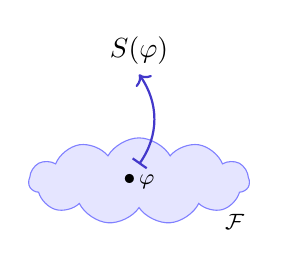
\begin{tikzpicture}[node distance=0.8cm]
        \node (target) {$S(\varphi)$};
        \node[draw=blue!50, fill=blue!10, cloud, cloud puffs=11, cloud puff arc=120, minimum width=2.8cm, minimum height=1.1cm, inner sep=0pt, below=of target] (F) {};
        \node[font=\footnotesize] (phi) at (F.center) {$\bullet\,\varphi$};
        \node[font=\footnotesize, anchor=north west] at ([xshift=6pt]F.south east) {$\mathcal{F}$};
        \draw[|->, thick, indigo] (phi.north) to[bend right=35] (target.south);
      \end{tikzpicture}
    \end{column}
  \end{columns}

  変分を取って \textbf{部分積分}  \begin{align*}
    \delta S &= \int_{-\infty}^{\infty} \left[\dot{\varphi}\,\delta\bar{\dot{\varphi}} + \bar{\dot{\varphi}}\,\delta\dot{\varphi} - \varphi\delta\bar{\varphi} - \bar{\varphi}\delta\varphi\right] dt \\
    &= -\int_{-\infty}^{\infty} \left[(\ddot{\varphi} + \varphi)\, \delta\bar{\varphi} + \overline{(\ddot{\varphi} + \varphi)}\, \delta\varphi \right] dt + \underbrace{\Bigl[\underbrace{\dot{\varphi}\,\delta\bar{\varphi} + \bar{\dot{\varphi}}\,\delta\varphi}_{=:\,\gamma}\Bigr]_{-\infty}^{\infty}}_{= 0}
  \end{align*}

  $\delta S = 0$ となるのは \hl{\ddot{\varphi} + \varphi = 0} $\leftarrow$ \textbf{クライン-ゴルドン方程式}
\end{frame}

\begin{frame}{解空間とシンプレクティック形式}
  \textbf{クライン-ゴルドン方程式の解空間} は
  \begin{center}\hl{\mathrm{Sol} \coloneqq \{ \varphi \mid \ddot{\varphi} + \varphi = 0 \} = \{ pe^{it} + qe^{-it} \mid p, q \in \mathbb{C} \}}\end{center}

  先ほどの $\gamma$ をさらに微分する（幾何的には曲率の計算）
  \[ \omega \coloneqq \delta\gamma = \delta\dot{\varphi} \wedge \delta\bar{\varphi} + \delta\bar{\dot{\varphi}} \wedge \delta\varphi \]

  $\mathrm{Sol}$ の条件 $\varphi = pe^{it} + qe^{-it}$ を代入して
  \begin{center}\hl{\omega_\mathrm{Sol} \coloneqq 2i(dp \wedge d\bar{p} - dq \wedge d\bar{q})} \quad $\leftarrow$ $\mathrm{Sol}$ 上の \textbf{シンプレクティック形式}\end{center}

  \vfill
  \begin{center}
  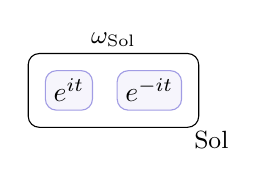
\begin{tikzpicture}[node distance=0.3cm, chipbox/.style={draw=indigo!50, fill=indigo!5, rounded corners, inner sep=3pt}]
    \node[chipbox] (s0) {$e^{it}$};
    \node[chipbox, right=of s0] (s1) {$e^{-it}$};
    \node[draw, rounded corners, fit=(s0)(s1), inner sep=6pt] (souter) {};
    \node[anchor=south, font=\small, inner sep=2pt] at (souter.north) {$\omega_\mathrm{Sol}$};
    \node[anchor=north west, font=\small, inner sep=1pt] at ([xshift=-3pt]souter.south east) {$\mathrm{Sol}$};
  \end{tikzpicture}
  \end{center}
\end{frame}

\begin{frame}{場の量子論とは}
  場の量子論は次の \textbf{2 つの組} で構成される
  \begin{center}ヒルベルト空間 \hl{\mathcal{H}}\end{center}
  \vspace{-0.4em}
  \begin{center}場の演算子 \hl{\Phi(s): \mathbb{R} \to \mathcal{E}\mathrm{nd}(\mathcal{H})}\end{center}
  \vspace{-1em}
  \begin{center}
  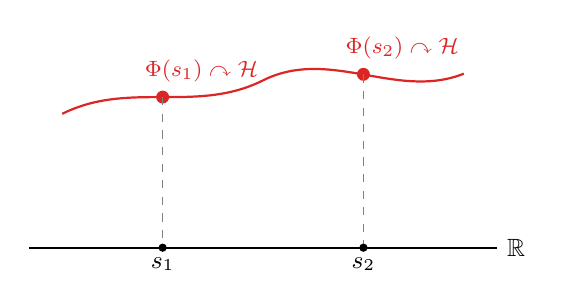
\begin{tikzpicture}[scale=0.85]
    \draw[thick, iotared]
      (-1, 2) .. controls (0, 2.5) and (1, 2) .. (2, 2.5)
              .. controls (3, 3) and (4, 2.2) .. (5, 2.6);
    \filldraw[iotared] (0.5, 2.25) circle (2.5pt);
    \node[iotared, font=\footnotesize, above=2pt of {(0.5, 2.25)}, xshift=14pt] {$\Phi(s_1) \curvearrowright \mathcal{H}$};
    \draw[dashed, gray] (0.5, 2.25) -- (0.5, 0);
    \filldraw[iotared] (3.5, 2.59) circle (2.5pt);
    \node[iotared, font=\footnotesize, above=2pt of {(3.5, 2.59)}, xshift=14pt] {$\Phi(s_2) \curvearrowright \mathcal{H}$};
    \draw[dashed, gray] (3.5, 2.59) -- (3.5, 0);
    \draw[thick] (-1.5, 0) -- (5.5, 0);
    \node[right, font=\small] at (5.5, 0) {$\mathbb{R}$};
    \filldraw (0.5, 0) circle (1.5pt);
    \node[below, font=\small] at (0.5, 0) {$s_1$};
    \filldraw (3.5, 0) circle (1.5pt);
    \node[below, font=\small] at (3.5, 0) {$s_2$};
  \end{tikzpicture}
  \end{center}
\end{frame}

\begin{frame}{場の量子論の構成}
  \vspace*{\fill}
  \begin{columns}[T]
    \begin{column}{0.56\textwidth}
      {\large\bfseries\color{indigo} ヒルベルト空間 $\mathcal{H}$}
      \par\bigskip

      $\mathrm{Sol}$ の \textbf{正エネルギー部分}

      \noindent
      \begin{minipage}[c]{0.7\columnwidth}
      \[ H_+ \coloneqq \{ pe^{it} \mid p \in \mathbb{C} \} \]
      \end{minipage}%
      \hfill
      \begin{minipage}[c]{0.25\columnwidth}
      \vspace{1pt}
      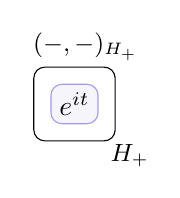
\begin{tikzpicture}[chipbox/.style={draw=indigo!50, fill=indigo!5, rounded corners, inner sep=3pt}]
        \node[chipbox] (h0) {$e^{it}$};
        \node[draw, rounded corners, fit=(h0), inner sep=6pt] (houter) {};
        \node[anchor=south, font=\small, inner sep=2pt] at ([xshift=4pt]houter.north) {$(-, -)_{H_+}$};
        \node[anchor=north west, font=\small, inner sep=1pt] at ([xshift=-3pt]houter.south east) {$H_+$};
      \end{tikzpicture}
      \end{minipage}

      \medskip
      シンプレクティック形式 $\omega_\mathrm{Sol}$ をひねると $H_+$ に \textbf{内積} $(-, -)_{H_+}$ が誘導される

      \bigskip
      \textbf{フォック空間} = \textbf{多項式環}

      \smallskip
      \noindent
      \begin{minipage}[c]{0.515\columnwidth}
      \hl{\mathcal{D} \coloneqq \bigoplus S^n H_+ = \mathbb{C}[e^{it}]}
      \end{minipage}%
      \hspace{6pt}%
      \begin{minipage}[c]{0.4\columnwidth}
      \vspace{8pt}
      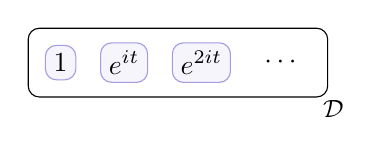
\begin{tikzpicture}[node distance=0.3cm, chipbox/.style={draw=indigo!50, fill=indigo!5, rounded corners, inner sep=3pt}]
        \node[chipbox] (n0) {$1$};
        \node[chipbox, right=of n0] (n1) {$e^{it}$};
        \node[chipbox, right=of n1] (n2) {$e^{2it}$};
        \node[right=of n2] (n3) {$\cdots$};
        \node[draw, rounded corners, fit=(n0)(n3), inner sep=6pt] (outer) {};
        \node[anchor=north west, font=\small, inner sep=1pt] at ([xshift=-3pt]outer.south east) {$\mathcal{D}$};
      \end{tikzpicture}
      \end{minipage}

      \medskip
      $\mathcal{D}$ を完備化して $\mathcal{H} \coloneqq \widehat{\mathcal{D}}$
    \end{column}
    \begin{column}{0.01\textwidth}
      \rule{0.5pt}{7.5cm}
    \end{column}
    \begin{column}{0.38\textwidth}
      {\large\bfseries\color{indigo} 場の演算子 $\Phi(s)$}
      \par\bigskip

      \hl{\varepsilon\, e^{ikt} \coloneqq e^{i(k+1)t}} \hfill \textbf{生成演算子} ({\color{epsgreen}$\uparrow$})

      \smallskip
      \hl{\iota\, e^{ikt} \coloneqq k\, e^{i(k-1)t}} \hfill \textbf{消滅演算子} ({\color{iotared}$\downarrow$})

      \begin{center}
      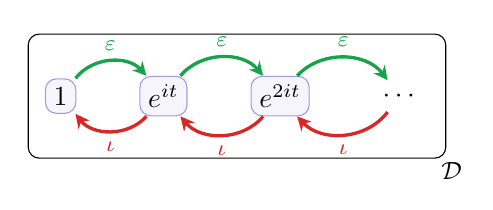
\begin{tikzpicture}[
        node distance=0.8cm,
        >={Stealth[length=5pt, width=5pt]},
        chipbox/.style={draw=indigo!50, fill=indigo!5, rounded corners, inner sep=3pt},
      ]
        \node[chipbox] (n0) {$1$};
        \node[chipbox, right=of n0] (n1) {$e^{it}$};
        \node[chipbox, right=of n1] (n2) {$e^{2it}$};
        \node[right=of n2] (n3) {$\cdots$};
        \draw[->, color=epsgreen, line width=1.2pt] (n0) to[bend left=50] node[above, font=\footnotesize, color=epsgreen] {$\varepsilon$} (n1);
        \draw[->, color=iotared, line width=1.2pt] (n1) to[bend left=50] node[below, font=\footnotesize, color=iotared] {$\iota$} (n0);
        \draw[->, color=epsgreen, line width=1.2pt] (n1) to[bend left=50] node[above, font=\footnotesize, color=epsgreen] {$\varepsilon$} (n2);
        \draw[->, color=iotared, line width=1.2pt] (n2) to[bend left=50] node[below, font=\footnotesize, color=iotared] {$\iota$} (n1);
        \draw[->, color=epsgreen, line width=1.2pt] (n2) to[bend left=50] node[above, font=\footnotesize, color=epsgreen] {$\varepsilon$} (n3);
        \draw[->, color=iotared, line width=1.2pt] (n3) to[bend left=50] node[below, font=\footnotesize, color=iotared] {$\iota$} (n2);
        \node[draw, rounded corners, fit=(n0)(n3), inner xsep=6pt, inner ysep=16pt] (outer) {};
        \node[anchor=north west, font=\small, inner sep=1pt] at ([xshift=-3pt]outer.south east) {$\mathcal{D}$};
      \end{tikzpicture}
      \end{center}

      \medskip
      \begin{center}\hl{\Phi(s) \coloneqq e^{is}\varepsilon + e^{-is}\iota}\end{center}
    \end{column}
  \end{columns}
  \vspace*{\fill}
\end{frame}

\begin{frame}{まとめ}
  \begin{center}
  \begin{tikzpicture}[arrlbl/.style={font=\scriptsize, midway, above}]
    \node[fill=hilight, rounded corners, inner sep=5pt] (S) {$S$};
    \node[right=1.5cm of S, fill=hilight, rounded corners, inner sep=5pt] (EM) {運動方程式};
    \node[right=1.5cm of EM, fill=hilight, rounded corners, inner sep=5pt] (Sol) {$(\mathrm{Sol}, \omega_\mathrm{Sol})$};
    \node[right=1.5cm of Sol, fill=hilight, rounded corners, inner sep=5pt] (HPhi) {$\mathcal{H}, \Phi(s)$};
    \draw[->] (S) -- node[arrlbl] {$\delta S = 0$} (EM);
    \draw[->] (EM) -- node[arrlbl] {$\gamma, \omega$} (Sol);
    \draw[->] (Sol) -- node[arrlbl] {$H_+, \mathbb{C}[e^{it}]$} (HPhi);
  \end{tikzpicture}
  \end{center}

  と場の量子論を構成できた。と思いきや、時空に空間がない\mbox{（$1+0$ 次元）}ので
  \begin{center}\large \textbf{量子力学 の範疇でした〜}\end{center}

  \medskip
  \noindent
  \begin{minipage}[c]{0.5\textwidth}
    \large でも、空間ありで同じ手順が可能で\\[4pt]
    {\Large\bfseries\color{indigo} 本物の場の量子論が作れます！}
  \end{minipage}\hfill
  \begin{minipage}[c]{0.45\textwidth}
  \centering
  \begin{tikzpicture}[scale=0.55]
    \draw[thick, iotared]
      (-1, 2) .. controls (0, 2.5) and (1, 2) .. (2, 2.5)
              .. controls (3, 3) and (4, 2.2) .. (5, 2.6);
    \filldraw[iotared] (0.5, 2.25) circle (2.5pt);
    \node[iotared, font=\scriptsize, above=2pt of {(0.5, 2.25)}, xshift=4pt] {$\Phi(s_1, x_1) \curvearrowright \mathcal{H}$};
    \draw[|->, gray, dashed] (0.1, 0.05) to[bend left=25] (0.4, 2.15);
    \filldraw[iotared] (3.5, 2.59) circle (2.5pt);
    \node[iotared, font=\scriptsize, above=2pt of {(3.5, 2.59)}, xshift=22pt] {$\Phi(s_2, x_2) \curvearrowright \mathcal{H}$};
    \draw[|->, gray, dashed] (3.9, -0.2) to[bend right=25] (3.6, 2.5);
    \draw[thick] (2, 0) ellipse (4.6 and 1.1);
    \node[anchor=north west, font=\scriptsize, inner sep=1pt] at ([xshift=-14pt, yshift=8pt]6.6, -1.1) {時空};
    \filldraw (0.5, 0.1) circle (1.5pt);
    \node[font=\scriptsize, below=1pt of {(0.5, 0.1)}] {$(s_1, x_1)$};
    \filldraw (3.5, -0.15) circle (1.5pt);
    \node[font=\scriptsize, below=1pt of {(3.5, -0.15)}] {$(s_2, x_2)$};
  \end{tikzpicture}
  \end{minipage}

  \vspace*{\fill}
  \vspace{1em}
  {\footnotesize\textbf{参考文献}: P. Deligne, P. Etingof, D. S. Freed, L. C. Jeffrey, D. Kazhdan, J. W. Morgan, D. R. Morrison, and E. Witten (eds.), \emph{Quantum Fields and Strings: A Course for Mathematicians, Vol. 1}, AMS, 1999.\par}
\end{frame}

\end{document}
